When reaching the camera sensor, the IR photons induce a current. The software interprets this signal and displays the corresponding temperature. According to the user's manual, these computations are based on equation \eqref{eq:powerTemp} (see section \ref{sec:theory}). As described in section \ref{sec:theory}, we are not yet able to reproduce the camera data with it. \\


To gain confidence in the software nevertheless and intuition for crucial variables in infrared measurements, we conducted studies using the camera software. Figure \ref{fig:softwareClean} shows the result. To obtain it, we took one of the thermograms taken during the emissivity measurements described in section \ref{sec:emissivityMeasurement} and chose one measurement point (paint right). We then manually set different ambient temperatures and varied for each of them the emissivity, keeping all other variables constant. In brief, the plot shows the dependence of the object temperature on ambient temperature and emissivity.
\todo[noline]{Find out at what temperature the thermogram was taken.}
\begin{figure}[h!]
	\centering
	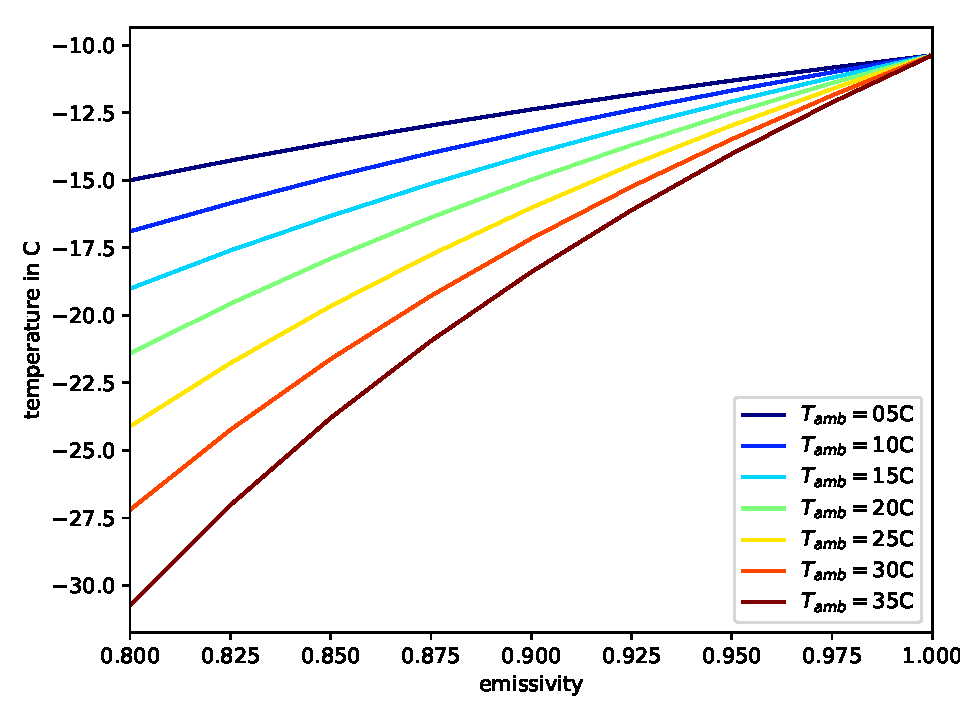
\includegraphics[width=0.7\textwidth]{img/softwareClean.pdf}
	\caption{Object temperature on the paint for different emissivities and ambient temperatures computed by the software.}
	\label{fig:softwareClean}
\end{figure}


Figure \ref{fig:softwareTape} shows the same plot using the same thermogram but using tape right as measurement point. As pointed out by the red dotted line, the emissivity for this measurement with real $T_\text{amb}=\SI{21.9}{\degreeCelsius}$ and real surface temperature $T_\text{pt100} = \SI{-11.54}{\degreeCelsius}$ should roughly be \SI{0.96}{}. This is close but not identical to the manufacturer value of \SI{0.95}{}. Thus, we can trust the measurement reasonably but there is either still some aspect of the measurement we do not understand or a small error in the software we need to determine.
\begin{figure}[h!]
	\centering
	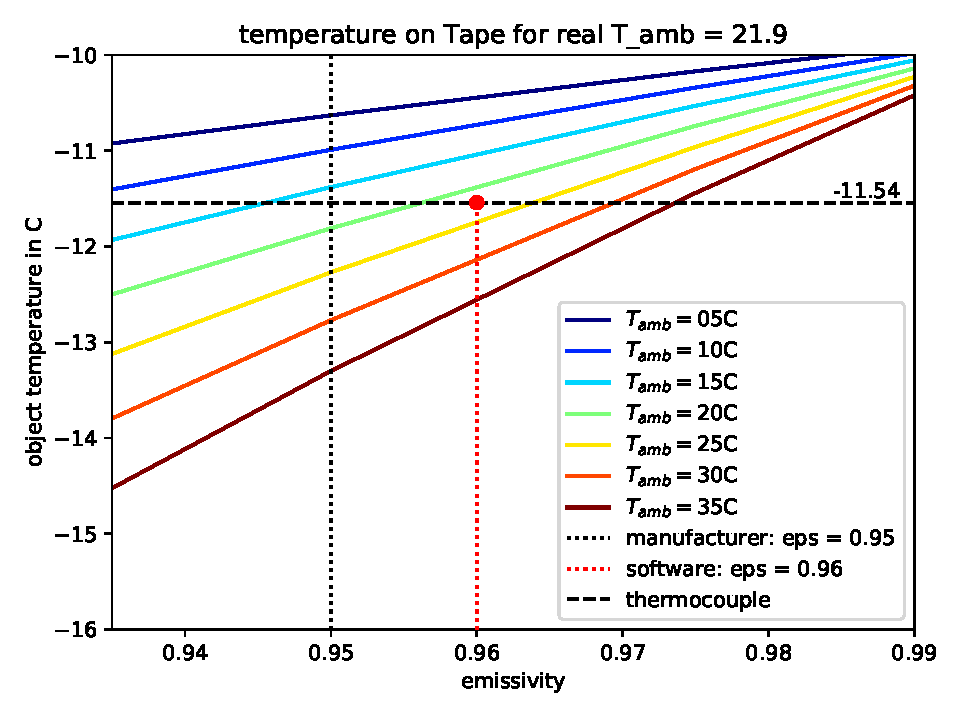
\includegraphics[width=0.7\textwidth]{img/softwareTape.pdf}
	\caption{Object temperature on the tape for different emissivities and ambient temperatures computed by the software.}
	\label{fig:softwareTape}
\end{figure} \\


If we go back to the paint, we can use this kind of plot to evaluate the impact of the uncertainty in the emissivity value (see section \ref{sec:emissivityMeasurement}) on the temperature measurement. Figure \ref{fig:softwarePaint-10} shows again the dependency of temperature on the paint on ambient temperature and emissivity. Assuming $T_\text{amb}=\SI{20}{\degreeCelsius}$, the emissivity range and the following temperature range is being highlighted by the orange dotted lines. More precisely, the emissivity range of $0.905\leq\epsilon\leq0.930$ determined in section \ref{sec:emissivityMeasurement} leads to a temperature uncertainty of just above \SI{1}{\degreeCelsius} at a real surface temperature of roughly $T_\text{pt100} = \SI{-10}{\degreeCelsius}$ (see \ref{fig:softwarePaint-10}). For colder temperatures around $T_\text{pt100} = \SI{-20}{\degreeCelsius}$, the following temperature uncertainty rises to \SI{2}{\degreeCelsius} (see \ref{fig:softwarePaint-20}. To accomplish the uncertainty threshold of \SI{1}{\degreeCelsius} on the temperature measurement in all temperature ranges, we need to restrict the emissivity some more.
\begin{figure}[h!]
	\centering
	\begin{subfigure}{0.7\textwidth}
		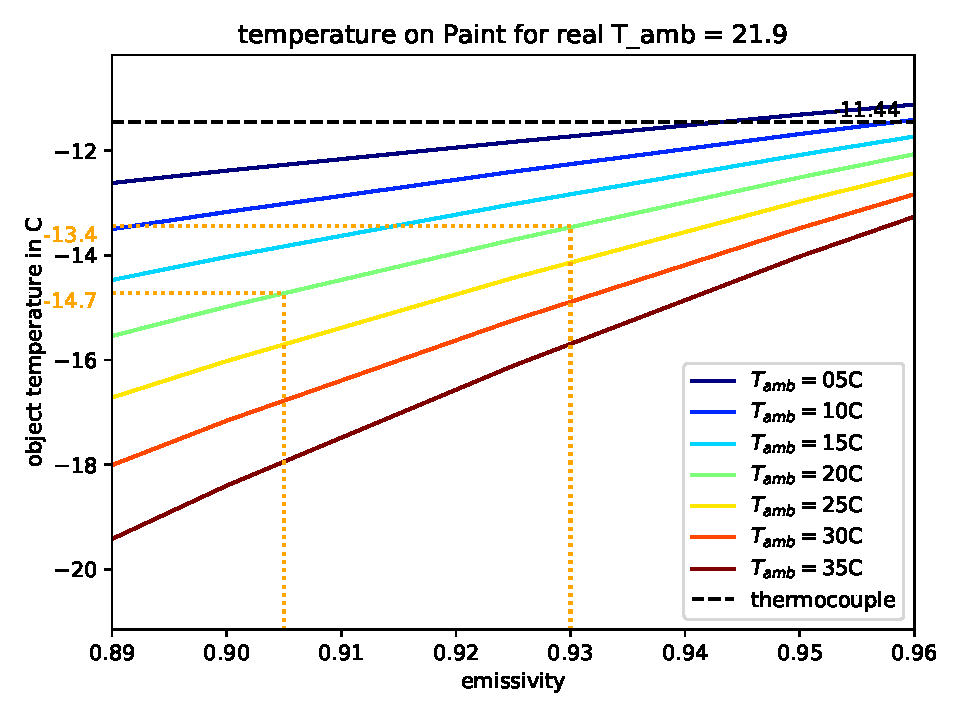
\includegraphics[width=\textwidth]{img/softwarePaint-10.pdf}
		\caption{$T_\text{pt100} = \SI{-11.44}{\degreeCelsius}$.}
		\label{fig:softwarePaint-10}
	\end{subfigure}
	\begin{subfigure}{0.7\textwidth}
		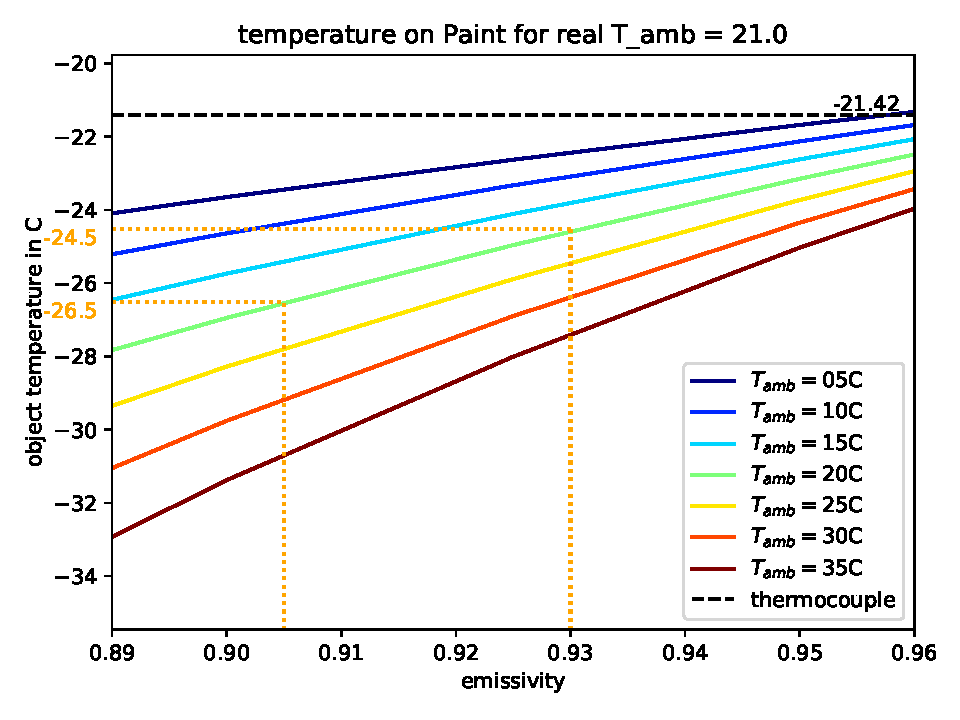
\includegraphics[width=\textwidth]{img/softwarePaint-20.pdf}
		\caption{$T_\text{pt100} = \SI{-21.42}{\degreeCelsius}$.}
		\label{fig:softwarePaint-20}
	\end{subfigure}
	\caption{Object temperature on the paint for different emissivities and ambient temperatures computed by the software, including a display of the effect of an uncertainty in the emissivity on the temperature for an ambient temperature of \SI{20}{\degreeCelsius}.}
	\label{fig:softwarePaint}
\end{figure}